\section{Conflict resolution at a glance}\index{Conflict resolution}

Whenever characters encounter an obstacle—be it an unsolvable riddle, a desperate struggle to escape a flooded sewer or a battle against a coven of deadly necromancers—they must find a way to overcome the challenge. Whether through wit, skill, or sheer determination, resolving conflicts is at the heart of the game, driving the story forward and shaping the fate of the characters.

With The Wyrd Engine, all conflict resolution follows the same pattern that combines \textbf{4dF} Fudge Dice, described \pagereftext{core:fudge-dice}, \textbf{Skills} described on \pagereftext{core:skills}, and \textbf{Traits} described on \pagereftext{core:traits}. You combine these three and compare them to a \textbf{Difficulty Rating (DR)}, described on \pagereftext{core:difficulty-rating}, and the result determines the outcome of a conflict.

\begin{DndReadAloud}{Steps in conflict resolution}
	\begin{itemize}
		\item Roll four Fudge Dice (\textbf{4dF}).
		      Each die has \textbf{+ (plus), - (minus), and 0 (blank) faces}. Add up the plusses and minuses.
		\item The roll result is added to a relevant \textbf{Skill} modifier.
		\item If relevant, \textbf{Traits} can be applied as bonuses.
		\item The final result is compared against a \textbf{difficulty rating (DR)} to determine success or failure:
		\begin{itemize}
			\item \textbf{4dF} + \textbf{Skill} + \textbf{Trait} $>$ \textbf{DR} (Success)	
			\item \textbf{4dF} + \textbf{Skill} + \textbf{Trait} $=$ \textbf{DR} (Tie)
			\item \textbf{4dF} + \textbf{Skill} + \textbf{Trait} $<$ \textbf{DR} (Failure)
		\end{itemize}
	\end{itemize}
\end{DndReadAloud}

This will always be the general pattern for resolving conflicts, only differing in which skills and traits are involved, how the difficulty rating is determined, and what the consequences of success or failure will be.

\section{Fudge dice (4dF)}\index{Fudge dice}\index{4dF}\label{core:fudge-dice}

Fudge dice are dice that can give you one of three values: \FudgeDie{-}, \FudgeDie{}, or \FudgeDie{+}. You can buy this type of dice if you want, but you can also use any normal six-sided die and declare 1 and 2 to be \FudgeDie{-}, 3 and 4 to be \FudgeDie{}, and 5 and 6. to be \FudgeDie{+}.

Whenever we roll dice in The Wyrd Engine, we roll four such dice (we write it as 4dF) and we add up the result, where \FudgeDie{-} counts as -1, \FudgeDie{} as 0, and \FudgeDie{+} as +1. So, for example
	\FudgeRes{++-0} = +1 + 1 - 1 + 0 = 1
	and 
	\FudgeRes{-+--} = -1 + 1 - 1 - 1 = -2.

Using 4dF gives us a distribution of outcomes that look like this:
\begin{center}
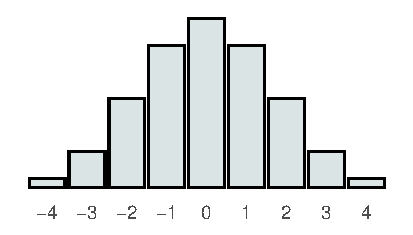
\includegraphics{stats/4dF.pdf}
\end{center}

You are unlikely to roll the extremes; you should expect to hit $\pm$4 about 1\% of the time (each)---about one time out of a hundred rolls, you should get +4, and about one time in a hundred, you should get -4. You expect to get an outcome above +3 or below -3 about 6\% of the time (each)---about one in twenty for each.

Another way to visualise the outcome of a 4dF is as the chance you have of rolling higher than some threshold value:

\begin{center}
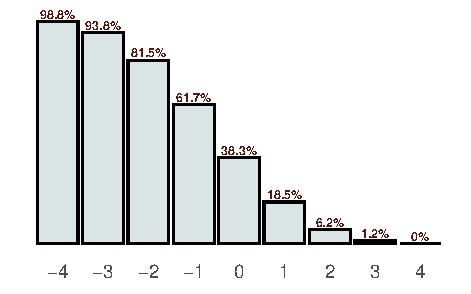
\includegraphics{stats/4dF-success.pdf}
\end{center}

To roll higher than \textbf{-4}, you just have to avoid \FudgeRes{----}, and this outcome only happens one out of 81 rolls. To roll higher than \textbf{+3} you \emph{have} to roll \FudgeRes{++++}, which also happens with probability 1/81. To roll \emph{higher} than \textbf{+4} is impossible, since this it the highest value you can roll.

In conflict resolution, this graph is relevant as it tells us how likely it is for a character without the necessary skills and relevant traits to succeed at any given difficulty rating. It is this graph of success probabilities you should have in mind when setting difficulty levels, and we return to it later. The graph, as it is here, is the probabilities you get if you had to rely on 4dF alone, without any skills or traits.

